\documentclass[a4paper,11pt]{resume}
\usepackage[utf8]{inputenc}
\usepackage{graphicx}
\usepackage{amsmath}
\usepackage{float}
\usepackage[left=0.75in,top=0.75in,right=0.75in,bottom=0.7in]{geometry}
\usepackage{titling}
\usepackage{hyperref}
\newcommand{\subtitle}[1]{%
  \posttitle{%
    \par\end{center}
    \begin{center}\large#1\end{center}
    \vskip0.5em}%
}
\usepackage{atbegshi}
\AtBeginDocument{\AtBeginShipoutNext{\AtBeginShipoutDiscard}}
\usepackage{etoolbox}
\patchcmd{\thebibliography}{\section*{\refname}}{}{}{}

\title{Rube Goldberg Machine Simulation: Project Report}
\subtitle{CS 251. Software Systems Lab (Group 23 - Cipher)}
\author{\bf{Yogesh Kumar}  \\
	140050004   \\
	yogesheth@cse.iitb.ac.in \\
	\and 
	\bf{Utkarsh Gautam} \\
	140050009  \\
	iamutkarsh@cse.iitb.ac.in \\
    \and 
    \bf{Suman Swaroop} \\
    140050032  \\
    sswaroop@cse.iitb.ac.in \\
    }
\date{\today}

\begin{document}

\maketitle

\begin{rSection}{{\heading Introduction}}
\begin{rSubsection}{}{}{}{}
\item A Rube Goldberg machine is a deliberately over-engineered or overdone machine that performs a very simple task in a very complex fashion, usually including a chain reaction. In this project we have created a simulation of a Rube Goldberg machine we designed, in C++ using the Box2D library.
\item We have created a GUI interface for visualization of the simulation and a non-GUI version for analysis of code statistics. We profile the code using gprof, the inbuilt Linux profiling tool, in order to identify which part of the simulation is taking the maximum amount of time to execute. Using this information, we optimize the code.
\item In this report we have given a gist of our design, its salient features and working. \\

\end{rSubsection}
\end{rSection}

\begin{rSection}{{\heading Design of the Simulation}}
This section explains the original design planned in for the simulation, the final design prepared and the changes done. It reflects on the salient features of Box2D library we have utilized in our simulation and various important elements, which are a part of the simulation. The original design was created at the beginning of the course, when our knowledge of Box2D was much less. Thus the design was rather minimal. However, now that we have got to learn more about Box2D\cite{var4}, we have added a few more elements to the simulation design to make it more interesting. \\ \\
\begin{rSubsection}{{\heading 1. Proposed Design}}{}{}{}
\begin{figure}[H]
\centering
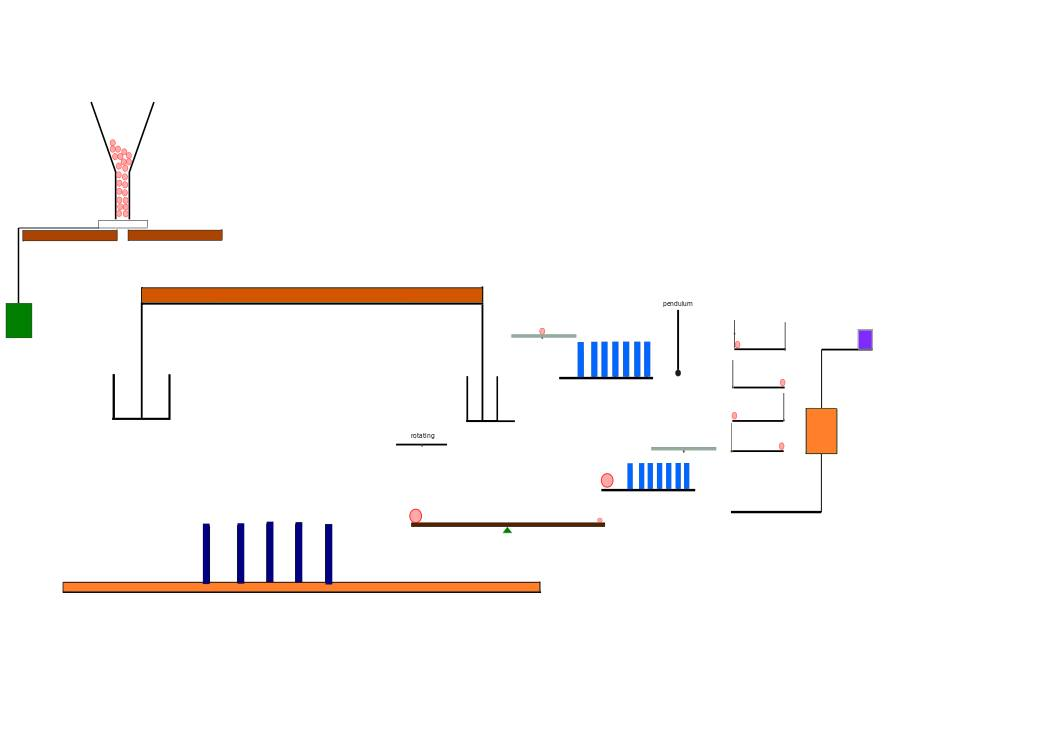
\includegraphics[width=0.6\textwidth]{init}
\label{fig:init}
\caption{Initial Design}
\end{figure}
\end{rSubsection}
\newpage
\begin{rSubsection}{{\heading 2. The Final Simulation Design}}{}{}{}
\begin{figure}[H]
\centering
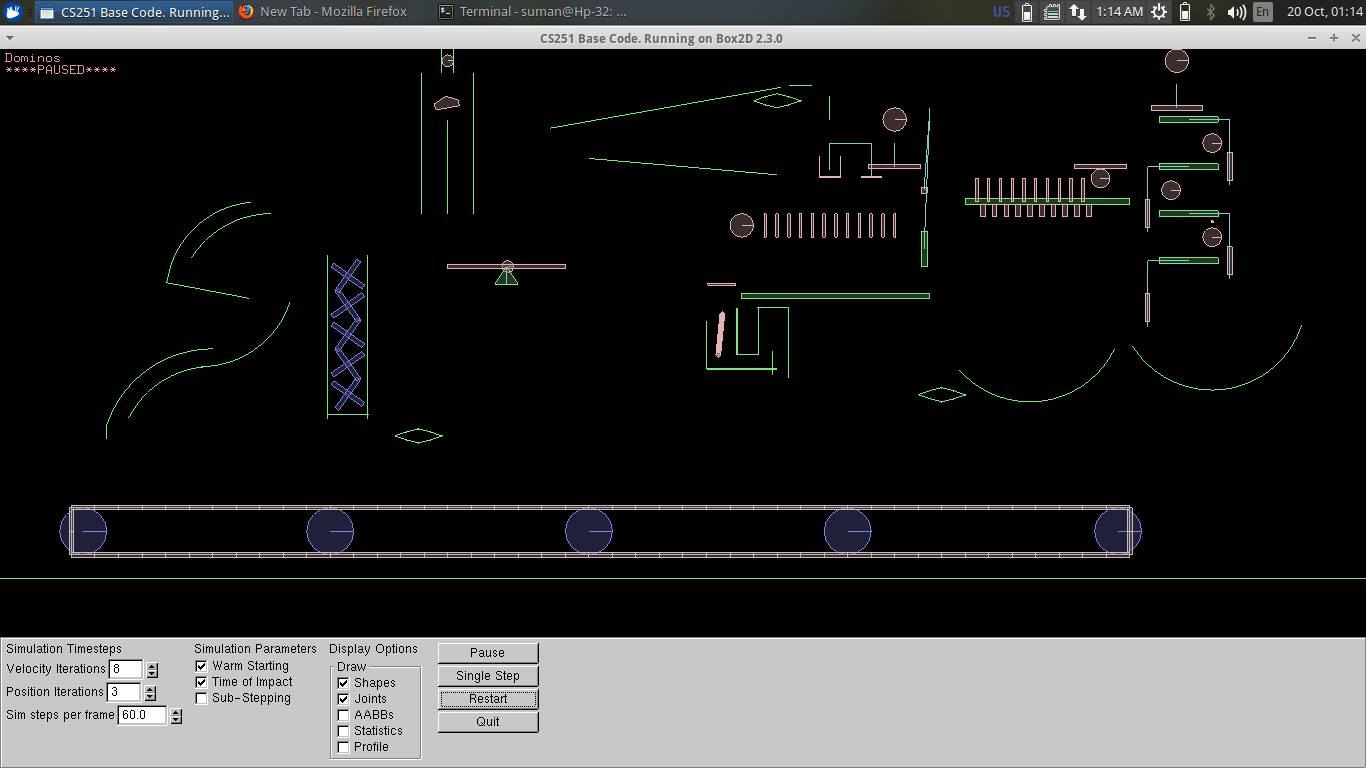
\includegraphics[width=0.6\textwidth]{screen.jpg}
\label{fig:find}
\caption{Final Design}
\end{figure}
The above image illustrates the original design planned for the simulation. The working of this design is as follows: 
\end{rSubsection}
\begin{rSubsection}{}{}{}{}
\vspace{-25pt}
\item The separator separates the 4 balls so that, 2 balls fall on the see saw system which throws 1 ball towards a teleporter on the right hand side and the other ball goes into the 5 gear peeler. 
\item The 2 other balls falls directly on the teleporter right below them which teleports them such that they fall in to the s shaped tube. The other ball which got teleported initiates the chain reaction in the set of dominoes which set free the balloon to trigger the system of rotating flaps.
\item The last ball from the system of rotating flaps falls into the beaker containing fluids which falls in the box containing the balls fell from the S shaped tube and moved towards the fluids by the conveyer belt. 
\end{rSubsection}

\begin{rSubsection}{{\heading Reasons for Deviation}}{}{}{}
As you might notice that our final implementation looks completely different from the proposed design. This is due to the fact that our TA's adivsed as to change and add a lot of objects as the initial design consisted of the objects provided in Outlab for LAB 03. We agreed to what our TA's were saying and started working on the project from a new aspect. 
\end{rSubsection}

\begin{rSubsection}{{\heading 3. Key Elements and Features}}{}{}{}
\begin{rSubsection}{{\heading 3.1 Separator}}{}{}{}
\\ \\
\begin{minipage}{0.15\textwidth}
\centering
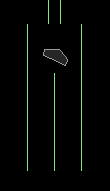
\includegraphics[width=0.6\textwidth,scale=0.4]{separator.png}
\label{fig:find}
\caption{Separator}
\end{minipage}
\begin{minipage}{0.80\textwidth}
Two Dividers plus a pentagon hinged at top to rotate about it.This is basically a pentagon polygon with fixed amount of rotating angle.
\end{minipage}
\\
\end{rSubsection}
\begin{rSubsection}{{\heading 3.2 Conveyer Belt}}{}{}{}
\\ \\

The belt is construct by a linked chain of rectangular segments, and wrapping it around some wheels to function as a belt. The belt is moved by turning the wheels. When two objects contact each other, the friction between them tries to stop their surfaces from moving relative to each other.The belt friction coefficient is set high.
\begin{figure}[h]
\centering
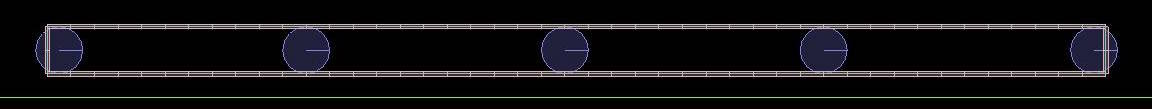
\includegraphics[width=0.8\textwidth]{conveyer.jpg}
\label{fig:find}
\caption{Conveyer Belt}
\end{figure}
\end{rSubsection}
\newpage
\begin{rSubsection}{{\heading 3.3 Teleporter}}{}{}{}
\begin{minipage}{0.15\textwidth}
\centering
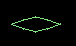
\includegraphics[width=\textwidth]{teleporter.png}
\label{fig:find}
\caption{Teleporter}

\end{minipage}
\begin{minipage}{0.80\textwidth}
This is a fictitious part of our project. We have used teleporter to move balls(fruits here) from one place to another. To implement this we overrided the b2ContactListener::BeginContact and EndContact functions. As soon a body touches the teleporter the mcontact bool variable becomes true and under step function of the base\underscoresim\underscoret class the code under the if condition runs and transforms the location of the body to another place(changing its properties).
\end{minipage}
\end{rSubsection}

\begin{rSubsection}{{\heading 3.4 Five Gear Peeler}}{}{}{}
\begin{minipage}{0.15\textwidth}
\centering
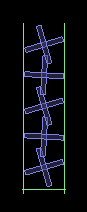
\includegraphics[width=0.6\textwidth,scale=0.4]{5gear.png}
\label{fig:find}
\caption{     Gear Peeler}
\end{minipage}
\begin{minipage}{0.80\textwidth}
The 3 fruit(balls here) plus one useless ball falling from the top. One of it enters the peeler. The peeler has 5 rotating gears that are set to same group index as not to collide with each other and are kinematic to rotate at same speed. They are fixed to that point by a joint to the base.
\end{minipage}
\end{rSubsection}

\begin{rSubsection}{{\heading 3.5 See-Saw System}}{}{}{}
\\ \\ 
It consists of a rectangular dynamic box and a triangular static wedge, which are connected by a revolute joint. The heavy sphere falls on one arm of the see saw and it rotates , thereby throws the ball on the other side of the see saw into the 5 gear elevator.
\end{rSubsection}

\begin{rSubsection}{{\heading 3.6 System of Rotating Flaps}}{}{}{}
\\ \\
\begin{minipage}{0.15\textwidth}
\centering
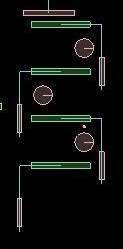
\includegraphics[width=0.6\textwidth,scale=0.4]{flaps.jpg}
\label{fig:find}
\caption{Rotating Flaps}
\end{minipage}
\begin{minipage}{0.80\textwidth}
 The system of rotating flags acts as a medium of momentum transfer from the top level to the bottom level. At each level, a sphere moves to the other end and hits the edge of the flap. Due to the motion of this flap, on the level below, a sphere is imparted momentum and its moves to the other end of the level and the same process repeats till the last sphere falls off the edge and hit the teleporter.
 \end{minipage}
\end{rSubsection}

\begin{rSubsection}{{\heading 3.7 Balloon}}{}{}{}
\\ \\
 We have used a balloon in the design. The balloon triggers the System of rotating flaps. The Balloon is a Box2D circle body, whose gravity has been scaled to a negative value.  
\end{rSubsection}

\begin{rSubsection}{}{}{}{}
\item \textbf{Use of \textit{SetGravityScale(..)} Function} : We have used the SetGravityScale(float) function of Box2D’s b2Body class. Using the function we can scale the gravity of any particular body to avalue of our choice. This is used to create objects like the balloons and the rocket. For the balloon, the gravity is scaled by −0.2. The low negative scale for the balloon make them seem to be rising with less acceleration like actual balloons would.
\end{rSubsection}

\end{rSection}
\newpage
\begin{rSection}{{\heading Code Profiling and Optimizations}}
\begin{rSubsection}{{\heading 1. Code Profiles}}{}{}{}

We profile the code with the profiler gprof and try to draw conclusions on the parts of the code that consume the most amount of time and calls. We have also figured out optimizations that can be carried out to improve the running time for the execution. We compile the code in debug and release versions (i.e. without or with −O3 flags) and examine the difference in profile outputs.
\begin{figure}[h]
\centering
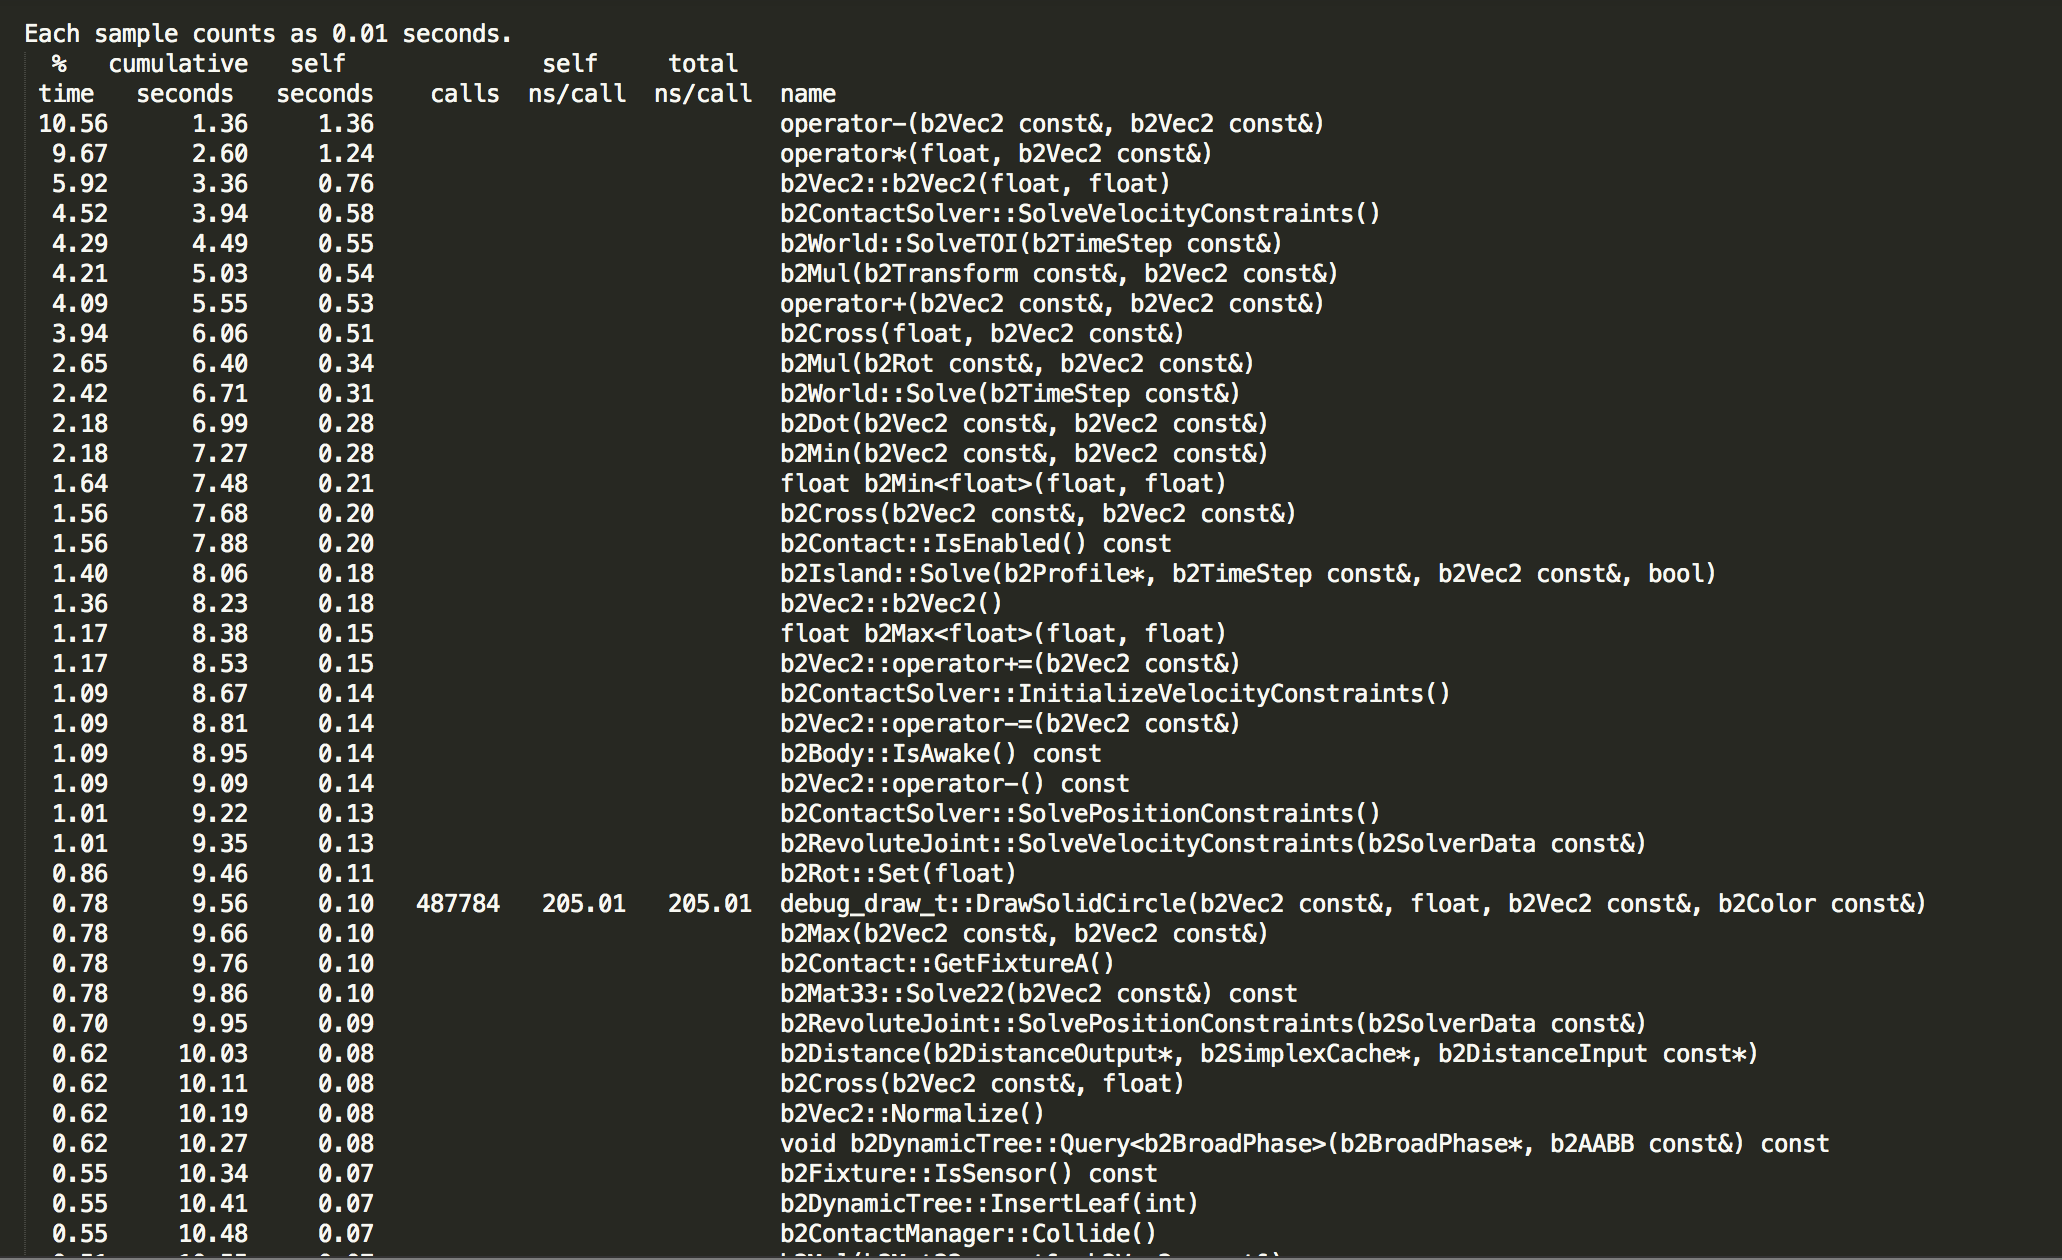
\includegraphics[width=0.86\textwidth]{debug}
\label{fig:init}
\caption{Profiling Output for Debug Version}
\end{figure}
\begin{figure}[h]
\centering
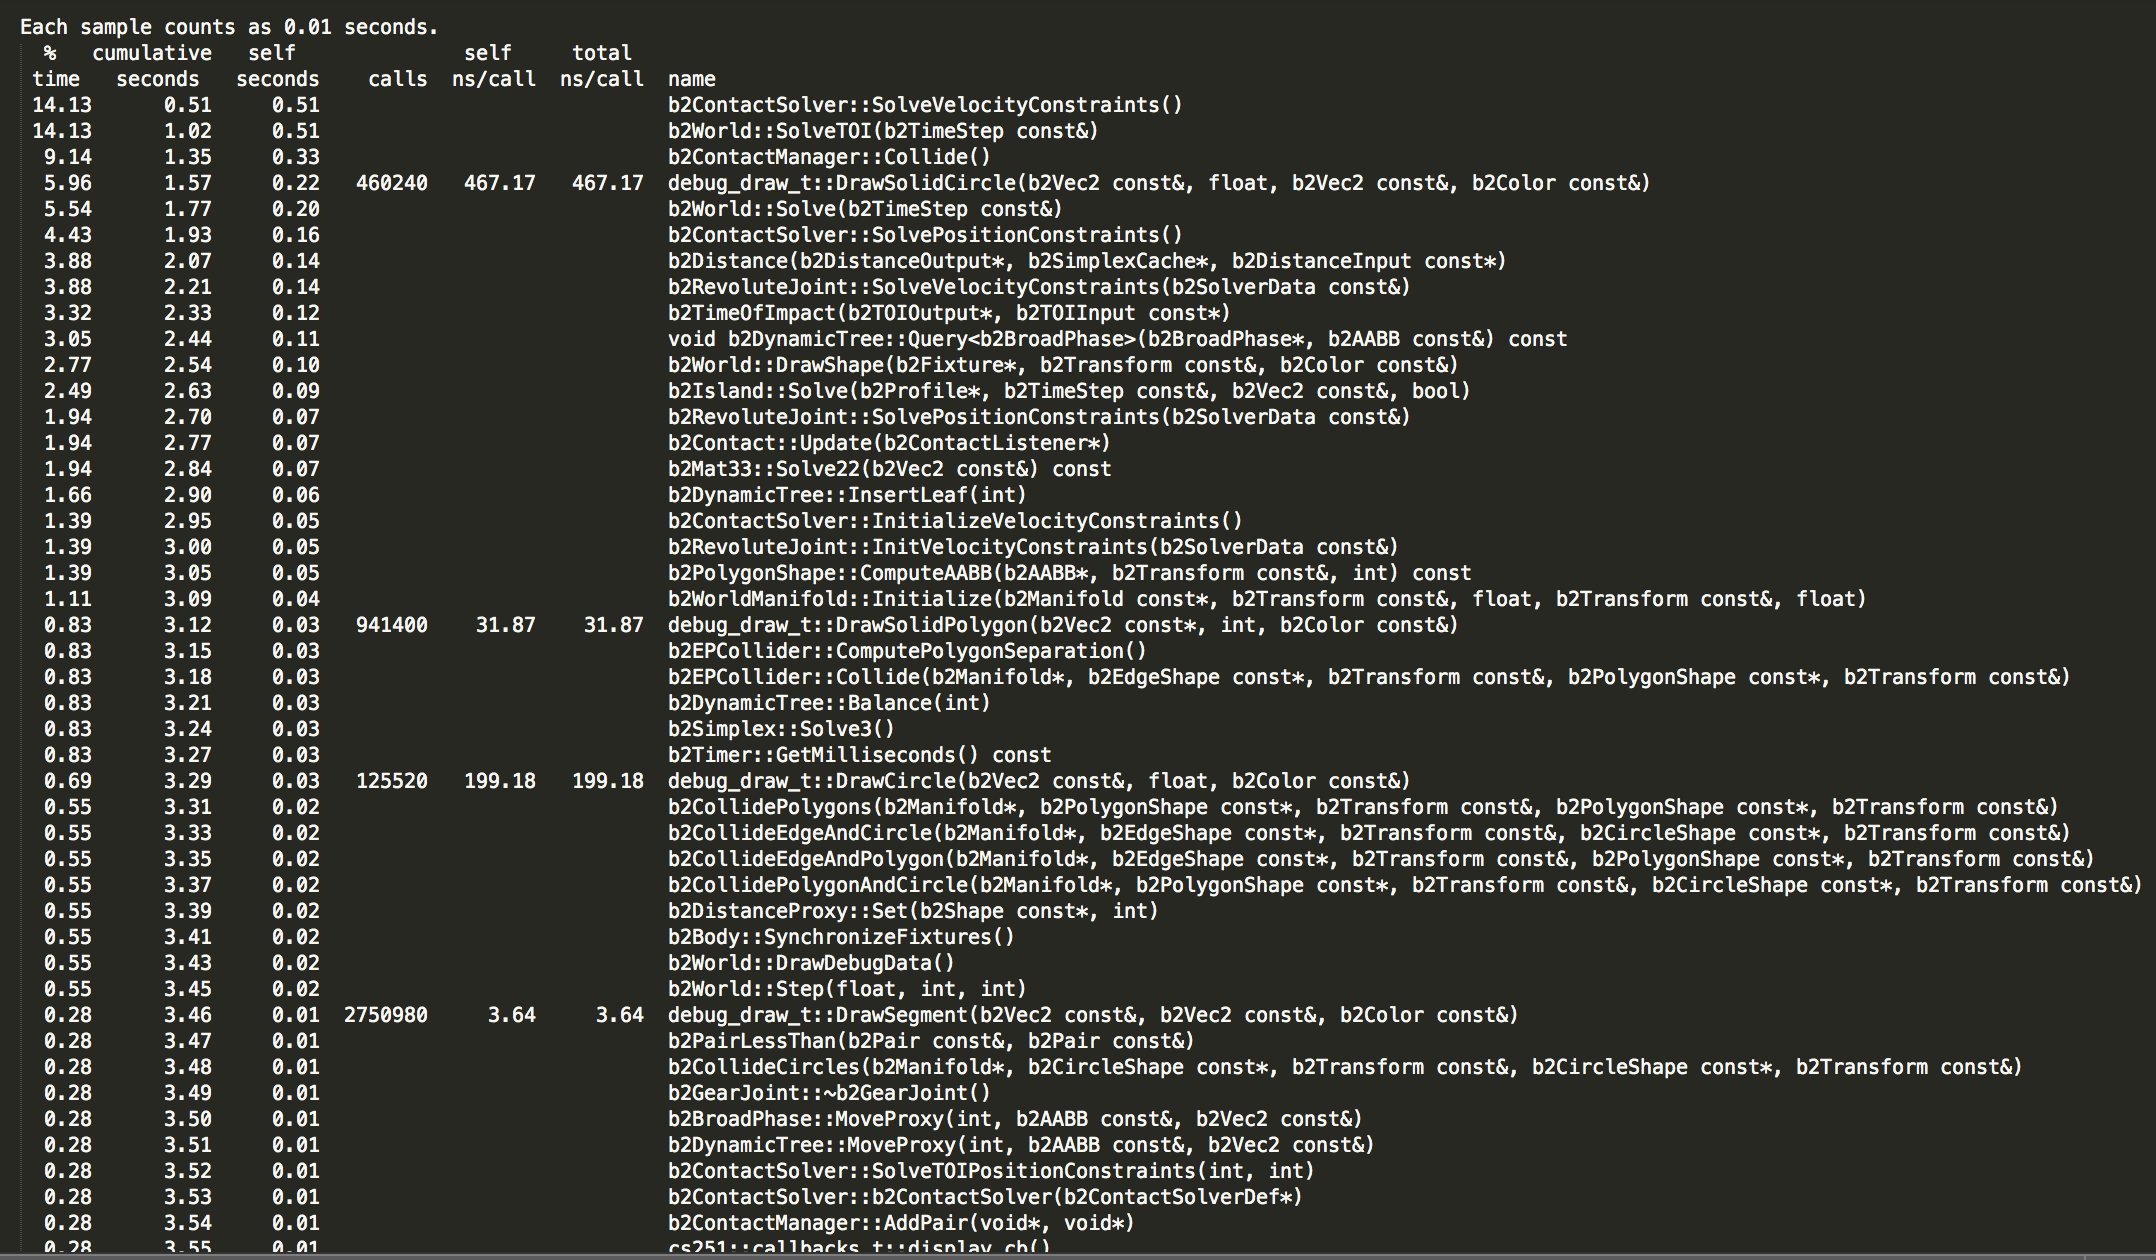
\includegraphics[width=0.86\textwidth]{release}
\label{fig:init}
\caption{Profiling Data for Release Version}
\end{figure}
\end{rSubsection}
\newpage
\begin{rSubsection}{{\heading 2. Optimizations}}{}{}{}
We now list some optimiztions that can be carried to improve the code:
\\ \\ \\
\begin{rSubsection}{{\heading 2.1 Debug Version}}{}{}{}
\\ \\
\textbf{operator+(b2Vec2const\&, b2Vec2const\&)} : \\
Debug Time : 0.53;  \\ \\
\textbf{floatb2Max\textless  float\textgreater (float, float)} : \\ 
Debug Time : 0.15; \\ \\
\textbf{operator\text{*}(float, b2Vec2const\&) } : \\
Debug Time : 1.24; 
\\ \\
\begin{rSubsection}{}{}{}{}
These overloaded operators perform operations on the vectors. Since,they are called a large amount of times, and each function call adds to the program time, as the program has to remember the program environment and pass the parameters by reference. Due to the large amount of calls, this adds up to significant time in the debug version. In the release version, these operators are totally eliminated as they are converted to inline functions by the - \textbf{finline-functions} flag (The compiler heuristically decides which functions are worth integrating in this way). Inline functions are implemented by copying the code in the function itself. This reduces the time of passing the parameters and reduces the overall time of the program.
\\
\end{rSubsection}
\end{rSubsection}
\begin{rSubsection}{{\heading 2.2 Debug Version}}{}{}{}
\\
\textbf{b2ContactSolver::SolveVelocityConstraints() }\\
Debug Time : 0.58; Release Time : 0.51 \\ \\
\textbf{b2ContactSolver::InitializeVelocityConstraints() } \\
Debug Time : 0.14; Release Time : 0.05 \\ \\
The Flag \textbf{-fprefetch-loop-arrays} (generate instructions to prefetch memory to improve the performance of loops that access large arrays.) and \textbf{-fpredictive-commoning} (from −O3) optimises this part of the code. \\ \\
\end{rSubsection}
\begin{rSubsection}{{\heading 2.3 Debug Version}}{}{}{}
\\
\textbf{b2Vec2::b2Vec2()} \\ 
\textbf{b2World::SolveTOI()} \\
Debug Time : 0.55; Release Time : 0.51 \\ \\
\item The number of calls to the b2Vec2 constructor is huge because this constructor is called everytime in the loop of SolveVelocityConstraints(). This can be optimised by defining the b2Vec2 outside the loop.
\item The release version performs this optimization. The number of calls of b2Vec2 constructor is reduced expotentially in the release version by defining the vectors outside the loop. This optimises a large amount of memory and time.
\end{rSubsection}
\end{rSubsection}
\newpage
\begin{rSubsection}{{\heading 3. Call Graphs}}{}{}{} 
\\
Call graphs are a way of analysing the function calls in the program. Call graphs show the call of functions in a function in the form of a graph. The children functions of a node are called in the function itself. \\
\begin{rSubsection}{{\heading Debug Version}}{}{}{}
\begin{figure}[h]
\centering
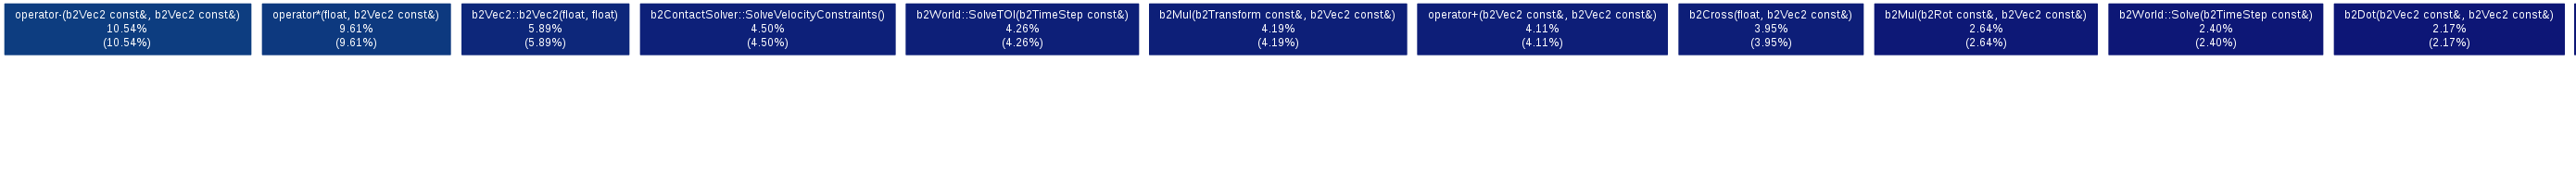
\includegraphics[width=0.86\textwidth]{analysisDebug}
\label{fig:init}
\caption{A Part of the Call Graph for the Debug Version}
\end{figure}
\end{rSubsection}
\begin{rSubsection}{{\heading Release Version}}{}{}{}
\begin{figure}[h]
\centering
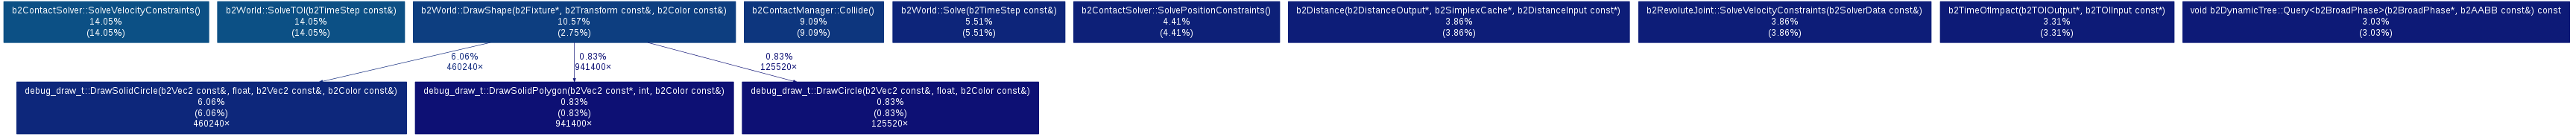
\includegraphics[width=0.86\textwidth]{releaseanalysis}
\label{fig:init}
\caption{A Part of the Call Graph for the Release Version}
\end{figure}
\end{rSubsection}
\end{rSubsection}
\begin{rSubsection}{{\heading Comparison with orignal call graph}}{}{}{}
Observation:\\
According to the base code  statistics operator - *, b2Distance, b2Min  function are taking maximum time.
But according to our project statistics b2SolveTOI, b2ContactManager, SolvePositionConstraints(),SolveVelocityConstraints() are taking maximum time.
Conclusion:\\
We have overrided contact function, step function and activated contact listener.So the cause of increased time of these function is that they are being called during each collision that occurs during BOX2D simulation and cross verifies with our conditions and accordingly carry out transformation in world which has increased their time from previous project.
\end{rSection}

\begin{rSection}{{\heading Difficulties Faced}}
The basic objects like circle, dominos, curved paths, pendulum were easy to make and was more or less have the same code style. \\
\begin{rSubsection}{{\heading All the Various Difficulties faced}}{}{}{}
\item Hydraulics: First we made very fine small circles to replicate drops and initialized 1000 of such balls.That caused segmentation fault(core dumped) quite often.
\item Teleporter: We had to implement b2ContactListener by overriding\: BeginContact and Endcontact functions.We faced difficulties in implementing the same in our project as our base code were predefined and was different from those given in online tutorials.
\item Time Synchronisation: This part was most difficult to make things occur in time one after other.
\end{rSubsection}
\begin{rSubsection}{{\heading Solution to Difficulties}}{}{}{}
\item Reduced the number of balls to 100.We increased the radius of balls and their restitution and still maintaining water like movement.
\item After Analysing all the provided source files, we were able to figure out the solution. We made the m\_world variable of test object public and set the onclicklistener for it in main.cpp file.
\item We took help of the teleporter(future fictitious object ) to move objects and conveyor belt speed which were changed in accordance whenever required.It was a trial and error method , changing values and running simulation again and again.
\end{rSubsection}
\end{rSection}
\newpage
\begin{rSection}{{\heading Work Distruibution}} 
\\
\begin{rSubsection}{{\heading Yogesh Kumar}}{}{}{}
\item Hydraulics, seperator in BOX2D simulation
\item Made report in latex, gprof call graphs.
\end{rSubsection}

\begin{rSubsection}{{\heading Utkarsh Gautam}}{}{}{}
\item Conveyor belt, bullet shoot in BOX2D simulation
\item Doxygen Documentation plus extra commenting the final codes.
\end{rSubsection}

\begin{rSubsection}{{\heading Suman Swaroop}}{}{}{}
\item Teleporter,curved paths,b2ContactListener overriding, Time Synchronisation(final step) in BOX2D
\item Made Beamer presentation and Makefile.
\\ \\
All other simple objects were made in presence of all of us so as to connect things up.
The pendulum, weight balancing pulley sytem, high restitution reflector, sphere bodies, dominos, curved paths. \\
\end{rSubsection}



\end{rSection}
\begin{rSection}{{\heading References}}
\\ \\
\begin{thebibliography}{9}
\bibitem{var1}
BOX2D manual\\
\url{www.iForce2d.net}
\bibitem{var2}
For error correction and debugging\\
\url{www.stackoverflow.com}
\bibitem{var3}
Conveyer belts:\\
\url{www.github.com/pratnala/cs296_spring2013/blob/master/src/dominos.cpp}
\bibitem{var4}
Some innovative ideas:
\url{https://www.youtube.com/watch?v=FZJOaY6Xh7Y}
\url{https://www.youtube.com/watch?v=Yv-aP53TdT4}
\bibitem{var5}
BOX2D Documentation\\
\url{www.box2d.org}
\bibitem{wiki1}
Rube Golberg Machine description:
\url{https://en.wikipedia.org/wiki/Rube_Goldberg_machine}
\end{rSection}
\end{document}
